\documentclass[10pt]{beamer}

\usepackage{helvet}
\usepackage{hyperref}
\usepackage{graphicx}
\usepackage{ulem}

\title{Introduction to Programming with Python}
\subtitle{Riding the Serpent}
\author{Anshul Nigham \& Rob Tirrell}
\date{\today}


\usetheme{Luebeck}
\hypersetup{
  pdftitle = \title,
  pdfauthor = {Rob Tirrell},
  pdfsubject = {Introduction to Programming with Python},
  colorlinks = true,
  urlcolor=blue
}

% Get rid of bottom navigation bars.
\setbeamertemplate{footline}[page number]{}

% Get rid of navigation symbols.
\setbeamertemplate{navigation symbols}{}


\usepackage{fancyvrb}
\usepackage{color}

\makeatletter
\def\PY@reset{\let\PY@it=\relax \let\PY@bf=\relax%
    \let\PY@ul=\relax \let\PY@tc=\relax%
    \let\PY@bc=\relax \let\PY@ff=\relax}
\def\PY@tok#1{\csname PY@tok@#1\endcsname}
\def\PY@toks#1+{\ifx\relax#1\empty\else%
    \PY@tok{#1}\expandafter\PY@toks\fi}
\def\PY@do#1{\PY@bc{\PY@tc{\PY@ul{%
    \PY@it{\PY@bf{\PY@ff{#1}}}}}}}
\def\PY#1#2{\PY@reset\PY@toks#1+\relax+\PY@do{#2}}

\def\PY@tok@gd{\def\PY@tc##1{\textcolor[rgb]{0.63,0.00,0.00}{##1}}}
\def\PY@tok@gu{\let\PY@bf=\textbf\def\PY@tc##1{\textcolor[rgb]{0.50,0.00,0.50}{##1}}}
\def\PY@tok@gt{\def\PY@tc##1{\textcolor[rgb]{0.00,0.25,0.82}{##1}}}
\def\PY@tok@gs{\let\PY@bf=\textbf}
\def\PY@tok@gr{\def\PY@tc##1{\textcolor[rgb]{1.00,0.00,0.00}{##1}}}
\def\PY@tok@cm{\let\PY@it=\textit\def\PY@tc##1{\textcolor[rgb]{0.25,0.50,0.50}{##1}}}
\def\PY@tok@vg{\def\PY@tc##1{\textcolor[rgb]{0.10,0.09,0.49}{##1}}}
\def\PY@tok@m{\def\PY@tc##1{\textcolor[rgb]{0.40,0.40,0.40}{##1}}}
\def\PY@tok@mh{\def\PY@tc##1{\textcolor[rgb]{0.40,0.40,0.40}{##1}}}
\def\PY@tok@go{\def\PY@tc##1{\textcolor[rgb]{0.50,0.50,0.50}{##1}}}
\def\PY@tok@ge{\let\PY@it=\textit}
\def\PY@tok@vc{\def\PY@tc##1{\textcolor[rgb]{0.10,0.09,0.49}{##1}}}
\def\PY@tok@il{\def\PY@tc##1{\textcolor[rgb]{0.40,0.40,0.40}{##1}}}
\def\PY@tok@cs{\let\PY@it=\textit\def\PY@tc##1{\textcolor[rgb]{0.25,0.50,0.50}{##1}}}
\def\PY@tok@cp{\def\PY@tc##1{\textcolor[rgb]{0.74,0.48,0.00}{##1}}}
\def\PY@tok@gi{\def\PY@tc##1{\textcolor[rgb]{0.00,0.63,0.00}{##1}}}
\def\PY@tok@gh{\let\PY@bf=\textbf\def\PY@tc##1{\textcolor[rgb]{0.00,0.00,0.50}{##1}}}
\def\PY@tok@ni{\let\PY@bf=\textbf\def\PY@tc##1{\textcolor[rgb]{0.60,0.60,0.60}{##1}}}
\def\PY@tok@nl{\def\PY@tc##1{\textcolor[rgb]{0.63,0.63,0.00}{##1}}}
\def\PY@tok@nn{\let\PY@bf=\textbf\def\PY@tc##1{\textcolor[rgb]{0.00,0.00,1.00}{##1}}}
\def\PY@tok@no{\def\PY@tc##1{\textcolor[rgb]{0.53,0.00,0.00}{##1}}}
\def\PY@tok@na{\def\PY@tc##1{\textcolor[rgb]{0.49,0.56,0.16}{##1}}}
\def\PY@tok@nb{\def\PY@tc##1{\textcolor[rgb]{0.00,0.50,0.00}{##1}}}
\def\PY@tok@nc{\let\PY@bf=\textbf\def\PY@tc##1{\textcolor[rgb]{0.00,0.00,1.00}{##1}}}
\def\PY@tok@nd{\def\PY@tc##1{\textcolor[rgb]{0.67,0.13,1.00}{##1}}}
\def\PY@tok@ne{\let\PY@bf=\textbf\def\PY@tc##1{\textcolor[rgb]{0.82,0.25,0.23}{##1}}}
\def\PY@tok@nf{\def\PY@tc##1{\textcolor[rgb]{0.00,0.00,1.00}{##1}}}
\def\PY@tok@si{\let\PY@bf=\textbf\def\PY@tc##1{\textcolor[rgb]{0.73,0.40,0.53}{##1}}}
\def\PY@tok@s2{\def\PY@tc##1{\textcolor[rgb]{0.73,0.13,0.13}{##1}}}
\def\PY@tok@vi{\def\PY@tc##1{\textcolor[rgb]{0.10,0.09,0.49}{##1}}}
\def\PY@tok@nt{\let\PY@bf=\textbf\def\PY@tc##1{\textcolor[rgb]{0.00,0.50,0.00}{##1}}}
\def\PY@tok@nv{\def\PY@tc##1{\textcolor[rgb]{0.10,0.09,0.49}{##1}}}
\def\PY@tok@s1{\def\PY@tc##1{\textcolor[rgb]{0.73,0.13,0.13}{##1}}}
\def\PY@tok@sh{\def\PY@tc##1{\textcolor[rgb]{0.73,0.13,0.13}{##1}}}
\def\PY@tok@sc{\def\PY@tc##1{\textcolor[rgb]{0.73,0.13,0.13}{##1}}}
\def\PY@tok@sx{\def\PY@tc##1{\textcolor[rgb]{0.00,0.50,0.00}{##1}}}
\def\PY@tok@bp{\def\PY@tc##1{\textcolor[rgb]{0.00,0.50,0.00}{##1}}}
\def\PY@tok@c1{\let\PY@it=\textit\def\PY@tc##1{\textcolor[rgb]{0.25,0.50,0.50}{##1}}}
\def\PY@tok@kc{\let\PY@bf=\textbf\def\PY@tc##1{\textcolor[rgb]{0.00,0.50,0.00}{##1}}}
\def\PY@tok@c{\let\PY@it=\textit\def\PY@tc##1{\textcolor[rgb]{0.25,0.50,0.50}{##1}}}
\def\PY@tok@mf{\def\PY@tc##1{\textcolor[rgb]{0.40,0.40,0.40}{##1}}}
\def\PY@tok@err{\def\PY@bc##1{\fcolorbox[rgb]{1.00,0.00,0.00}{1,1,1}{##1}}}
\def\PY@tok@kd{\let\PY@bf=\textbf\def\PY@tc##1{\textcolor[rgb]{0.00,0.50,0.00}{##1}}}
\def\PY@tok@ss{\def\PY@tc##1{\textcolor[rgb]{0.10,0.09,0.49}{##1}}}
\def\PY@tok@sr{\def\PY@tc##1{\textcolor[rgb]{0.73,0.40,0.53}{##1}}}
\def\PY@tok@mo{\def\PY@tc##1{\textcolor[rgb]{0.40,0.40,0.40}{##1}}}
\def\PY@tok@kn{\let\PY@bf=\textbf\def\PY@tc##1{\textcolor[rgb]{0.00,0.50,0.00}{##1}}}
\def\PY@tok@mi{\def\PY@tc##1{\textcolor[rgb]{0.40,0.40,0.40}{##1}}}
\def\PY@tok@gp{\let\PY@bf=\textbf\def\PY@tc##1{\textcolor[rgb]{0.00,0.00,0.50}{##1}}}
\def\PY@tok@o{\def\PY@tc##1{\textcolor[rgb]{0.40,0.40,0.40}{##1}}}
\def\PY@tok@kr{\let\PY@bf=\textbf\def\PY@tc##1{\textcolor[rgb]{0.00,0.50,0.00}{##1}}}
\def\PY@tok@s{\def\PY@tc##1{\textcolor[rgb]{0.73,0.13,0.13}{##1}}}
\def\PY@tok@kp{\def\PY@tc##1{\textcolor[rgb]{0.00,0.50,0.00}{##1}}}
\def\PY@tok@w{\def\PY@tc##1{\textcolor[rgb]{0.73,0.73,0.73}{##1}}}
\def\PY@tok@kt{\def\PY@tc##1{\textcolor[rgb]{0.69,0.00,0.25}{##1}}}
\def\PY@tok@ow{\let\PY@bf=\textbf\def\PY@tc##1{\textcolor[rgb]{0.67,0.13,1.00}{##1}}}
\def\PY@tok@sb{\def\PY@tc##1{\textcolor[rgb]{0.73,0.13,0.13}{##1}}}
\def\PY@tok@k{\let\PY@bf=\textbf\def\PY@tc##1{\textcolor[rgb]{0.00,0.50,0.00}{##1}}}
\def\PY@tok@se{\let\PY@bf=\textbf\def\PY@tc##1{\textcolor[rgb]{0.73,0.40,0.13}{##1}}}
\def\PY@tok@sd{\let\PY@it=\textit\def\PY@tc##1{\textcolor[rgb]{0.73,0.13,0.13}{##1}}}

\def\PYZbs{\char`\\}
\def\PYZus{\char`\_}
\def\PYZob{\char`\{}
\def\PYZcb{\char`\}}
\def\PYZca{\char`\^}
% for compatibility with earlier versions
\def\PYZat{@}
\def\PYZlb{[}
\def\PYZrb{]}
\makeatother


\begin{document}

\begin{frame}
  \titlepage
\end{frame}

\begin{frame}
  \small
  \frametitle{About Us}
  \begin{block}{Anshul Nigham}
    \begin{itemize}
      \item Began programming at 12 on on 8086 PC-XT (a full-fledged computer 20x slower than an iPhone).
      \item Converts caffeine into code for a living at Google.
    \end{itemize}
  \end{block}
  \begin{block}{Rob Tirrell}
    \begin{itemize}
      \item In the second year of a five to six year sentence in the Butte lab (\href{http://buttelab.stanford.edu/}{http://buttelab.stanford.edu/}), an entirely 'dry' lab (computers only -- the only other equipment necessary is a coffee machine).
      \item First language was Python, spends most days writing code in R, Python, Ruby and C++.
    \end{itemize}
  \end{block}
\end{frame}

\begin{frame}
  \frametitle{In Case of Emergency, Panic!}
  \begin{center}
    
\includegraphics[width=100px]{AlertSign.jpg}
  \end{center}
  \begin{itemize}
    \item But, really, please ask us questions -- raise your hand or whatever.
    \item As this is an introductory course, many of you will be wondering about the same things.
      Be a leader, just ask and Make Your Voice Heard.
  \end{itemize}
\end{frame}

\begin{frame}
  \frametitle{Principal Principles of Programming (1)}
  \begin{quote}
    \textbf{Computer programming} or \textbf{coding} is the process of designing, writing, testing, debugging/troubleshooting, and maintaining the source code of computer programs. 
    This source code is written in a programming language. The purpose of programming is to create a program that exhibits a certain desired behaviour. 
    The process of writing source code often requires expertise in many different subjects, including knowledge of the application domain, specialized algorithms and formal logic.
  \end{quote}
  \begin{flushright}
    \footnotesize -- Wikipedia
  \end{flushright}
\end{frame}

\begin{frame}
  \frametitle{Principal Principles of Programming (2)}
  \begin{quote}
    \footnotesize
    \sout{
      \textbf{Computer programming} or \textbf{coding} is the process of designing, writing, testing, debugging/troubleshooting, and maintaining the source code of computer programs. 
      This source code is written in a programming language. The purpose of programming is to create a program that exhibits a certain desired behaviour. 
      The process of writing source code often requires expertise in many different subjects, including knowledge of the application domain, specialized algorithms and formal logic.
    }
  \end{quote}
  \normalsize
  \begin{block}{The Heart of the Matter}
    \begin{itemize}
      \item While true, this definition is not particularly helpful, so we propose an alternative.
      \item At its core, programming is just writing a set of instructions which a computer runs on your behalf.
      \item How you conceive of and design those instructions is the fun part (and the challenge).
    \end{itemize}
  \end{block}
\end{frame}


\begin{frame}
  \frametitle{Principal Principles of Programming (3)}
  \begin{block}{Decomposition}
    \begin{itemize}
      \item \textbf{Decomposition} is the means by which a complex problem or system is broken down into parts that are easier to understand, program and maintain.
      \item This is one of the fundamental principles of design and programming: we decompose the logical structure into smaller, reusable units which we build one-at-a-time.
      \item Sometimes, how this decomposition should proceed isn't immediately clear.
        Then your first step should be thinking in depth about the problem you're facing, and in what ways it can be reduced into component subproblems.
    \end{itemize}
  \end{block}
\end{frame}

\begin{frame}
  \frametitle{Principal Principles of Programming (4)}
  \centering
  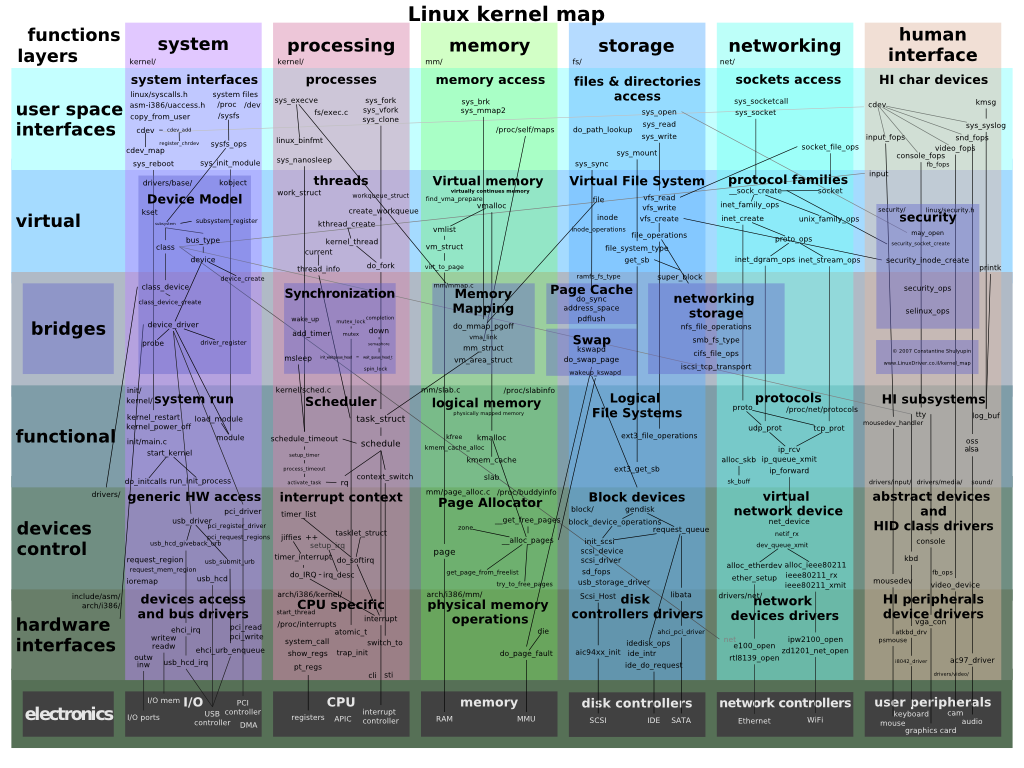
\includegraphics[width=300px]{LinuxKernelMap.png}
  \begin{flushright} 
    \footnotesize -- Wikipedia
  \end{flushright}
\end{frame}

\begin{frame}
  \frametitle{Principal Principles of Programming (5)}
  \begin{block}{Divide and Conquer}
    \begin{itemize}
      \item Imagine you are a pin manufacturer in 18th century England.
        To achieve maximum efficiency, you will make pins step-by-step: pounding the metal into a sheet, cutting the sheet into small strips, heating the protopins, elongating the pins, punching an eyelet, polishing the pins, etc..
      \item This is simple enough: just a stepwise series of transformations.
        More often, a computer program will be more complex, and have multiple interdependent parts.
    \end{itemize}
  \end{block}
\end{frame}

\begin{frame}
  \frametitle{Principal Principles of Programming (6)}
  \begin{block}{Motivating by Example}
    \centering
    \vspace{10px}
    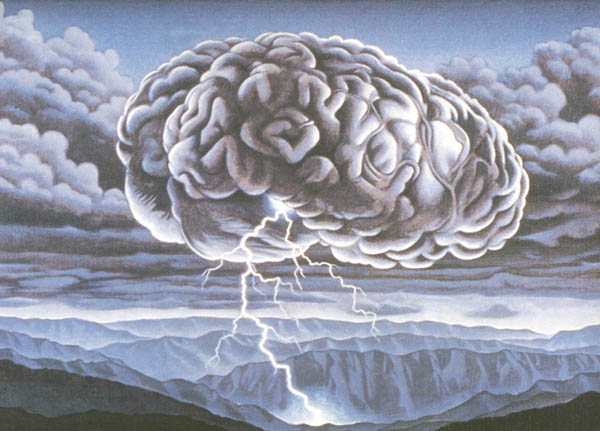
\includegraphics[width=125px]{Brainstorm.jpg}
    \vspace{5px}
    \begin{itemize}
      \item Think of an application you use frequently (a desktop application, a website, a phone application, etc.).
      \item What are the application and user operations we would want to support, and what are their requirements?
      \item With your nearest neighbors, consider and discuss how you would design this application.
        \textbf{Go!}
    \end{itemize}
  \end{block}
\end{frame}

\begin{frame}
  \frametitle{What is Python?}
  \centering
  
\includegraphics[scale=0.5]{PythonLogo.png} \\
  \begin{itemize}
    \item First released in 1991 by a Dutchman named Guido van Rossum (GvR).
    \item That's Self-Appointed Benevolent Dictator for Life (SABDFL) van Rossum to the rest of us.
    \item An interpreted, high-level language with flexible typing.
    \item Currently on its third major release... in other words, it's been around the block and has withstood the test of time.
  \end{itemize}
\end{frame}

\begin{frame}
  \frametitle{A Satisfied User}
  \begin{quote}
      Python has been an important part of Google since the beginning, and remains so as the system grows and evolves. Today dozens of Google engineers use Python, and we're looking for more people with skills in this language.
  \end{quote}
  \begin{flushright}
    \footnotesize
    -- Peter Norvig, Director of Search Quality at Google \\ and Computer Science Superstar
  \end{flushright}
\end{frame}

\begin{frame}
  \frametitle{Other Satisfied Users}
  \begin{itemize}
    \item \textbf{AstraZeneca} uses Python in drug discovery pipelines.
    \item \textbf{Phillips'} fabrication plants are managed in Python.
    \item \textbf{Industrial Light \& Magic} (Star Wars) employs Python for process management.
    \item \textbf{Anshul} developed an AdWords (Google's advertising platform) optimizer in Python.
    \item In \textbf{Rob's} work, people use Python at every point in the research pipeline (preprocessing and sanitization, standard analyses, data aggregation and integration, and so forth).
    \item It may be new to you, but according to TIOBE's programming languages index, Python is the sixth-most popular in the world.
    \item A list of anecdotes can't quite prove a point, so we'll try to justify why you should care about and use Python.
  \end{itemize}
\end{frame}

\begin{frame}
  \frametitle{Good for Them, What's in it for You?}
  \begin{block}{Power}
    \begin{itemize}
      \item Python facilitates rapid development.
        It comes with a huge collection of software (libraries) for many purposes.
      \item There is a sizeable, vibrant and very helpful Python community/ecosystem, should you run into trouble or seek advice.
    \end{itemize}
  \end{block}
  \begin{block}{Clarity}
    \begin{itemize}
      \item Python is remarkably clear and readable compared to many other languages.
      \item It actually takes some effort to write difficult-to-understand programs.
    \end{itemize}
  \end{block}
%  Before we can reveal Python, let's consider the high-level \textbf{process and principles of programming} (trust us, we know they're abstract and seemingly useless, but it's critical to really get what they mean).
\end{frame}

\begin{frame}
  \frametitle{The Interpreter (1)}
  \begin{block}{$>>>$}
    \begin{itemize}
      \item Python is an interpreted language.
        The computer reads, understands (compiles) and executes it on the fly, instead of reading and compiling ahead of time (as with C, C++, and many others).
      \item Because of this, we can use Python interactively, which is extremely helpful for designing and troubleshooting code.
    \end{itemize}
  \end{block}
  \begin{block}{IDLE}
    \begin{itemize}
      \item IDLE is Python's interpreter shell, which we'll use to walk through examples throughout the course.
      \item For those of you with Macs, you can open a Terminal and launch Python by typing \texttt{python}.
    \end{itemize}
  \end{block}
\end{frame}

\begin{frame}[fragile]
  \frametitle{The Interpreter (2)}
  \begin{block}{The \texttt{print} Function}
    \begin{itemize}
      \item Strings are surrounded by single (') or double (``) quotes, which are equivalent (but you must use the same type for any particular string).
        e.g., if you want a string to have a contraction, you can use double quotes to surround it, like \texttt{"The white whale mustn't breach, Moby is waiting."}.
      \item \texttt{print} is a core Python function, which by default outputs text to the screen. It's somewhat special, in that parentheses are optional when using (calling) it.
    \end{itemize}
  \end{block}
  \begin{block}{A Longstanding Tradition}
      Three equivalent \texttt{'Hello, World!'}s:
\begin{Verbatim}[commandchars=\\\{\}]
\PY{k}{print} \PY{l+s}{'}\PY{l+s}{Hello, World!}\PY{l+s}{'}
\PY{k}{print} \PY{l+s}{"}\PY{l+s}{Hello, World!}\PY{l+s}{"}
\PY{k}{print}\PY{p}{(}\PY{l+s}{'}\PY{l+s}{Hello, World!}\PY{l+s}{'}\PY{p}{)}
\end{Verbatim}
  \end{block}
\end{frame}

\begin{frame}
  \frametitle{The Interpreter (3)}
  \begin{block}{Not Your Daddy's Desktop Calculator}
    \begin{itemize}
      \item Among other uses, we can employ Python as a calculator.
      \item At the interpreter (\texttt{$>>>$}), type \texttt{4 + 2}.
        You should see \texttt{6}.
        So far, so good -- naturally, other operators are available (e.g. \texttt{+ - * /}).
    \end{itemize}
  \end{block}
  \begin{block}{Balling}
    \begin{itemize}
      \item To delve deeper into Python, we're going to work through a baseball\footnote{Baseball is a popular American sport. Rob's hometown is the supposed 'birthplace of baseball'.} statistics\footnote{The deliberate application of statistics to baseball is known as 'sabremetrics'. Check it out, it's really interesting.} example.
    \end{itemize}
  \end{block}
\end{frame}

\begin{frame}
  \frametitle{The Interpreter (4)}
  \begin{block}{Still Balling}
    \begin{itemize}
      \item A player's \textbf{slugging percentage} is calculated as \texttt{(singles + 2 * doubles + 3 * triples + 4 * homers) / at bats}.
        Basically, the numerator is the number of bases that player moves as a result of his offense.
      \item In \texttt{1920}, Babe Ruth appeared at the plate \texttt{458}\footnote{The divisor -- at bats -- needs to be a floating-point number, so enter it as \texttt{458.0}, otherwise Python will drop the fractional component of the result.  This behavior can be a pain, and has been changed in Python 3.} times, cranking out \texttt{73} singles, \texttt{36} doubles, \texttt{9} triples and \texttt{54} home runs.    
    \end{itemize}
  \end{block}
\end{frame}

\begin{frame}
  \frametitle{The Interpreter (5)}
  \begin{block}{More than a Glorified Calculator -- Saving it for Later}
    \begin{itemize}
      \item It can be tedious to have to type out that expression every time.
        Luckily for us and our fingers, we can store the results of calculations in \textbf{variables} very simply in Python.
      \item For example, \texttt{sp = (73 + 2 * 36 + 3 * 9 + 4 * 54) / 458.0}
        If you mess up the numbers, you can always try again.
        The new value will replace the old one.
      \item Voil\`{a}! Try \texttt{print}ing the result.
    \end{itemize}
  \end{block}
\end{frame}


\begin{frame}
  \frametitle{The Interpreter (6)}
  \begin{block}{Back to the Babe}
    \begin{itemize}
      \item Another useful stat is \texttt{on-base percentage} (OBP), calculated as \texttt{(H + BB + HBP) / (AB + BB + HBP + SF)}.  
        In English, \texttt{(hits + walks + hit by pitches) / (hits + walks + hit by pitches + sacrifice flies)}.
      \item In 1920, the Babe had \texttt{172} hits, walked \texttt{150} times, was hit by \texttt{3} pitches, and had no sacrifice flies (and \texttt{458} at bats).
        What was his OBP (hint: store this in a variable \texttt{obp})?
      \item \textbf{On-base plus slugging} (OPS) is a summary statistic frequently used to quantify players' offensive contributions.
        Since we have both of these measures already stored, calculating Ruth's OPS is as simple as \texttt{sp + obp}!
      \item Hopefully this illustrates the value of saving the results of intermediate computation.
        You'll thank yourself later.
    \end{itemize}
  \end{block}
\end{frame}

\begin{frame}
  \frametitle{Brief Interlude: Setting Up KomodoEdit}
  \begin{center}
    
\includegraphics[width=300px]{KomodoEdit.png}
  \end{center}
  \begin{itemize}
    \item KomodoEdit should already be installed on the provided computers, if not, visit \href{http://www.activestate.com/komodo-edit/downloads}{http://www.activestate.com/komodo-edit/downloads} to grab it.
  \end{itemize}
\end{frame}


\begin{frame}
  \frametitle{Playing Ball with Datatypes (1)}
  \begin{block}{What are They?}
    \begin{itemize}
      \item A \textbf{datatype} refers to a location in the computer's memory and the type of information stored there.
      \item Numbers can be of the \texttt{int} (integer) datatype, like \texttt{4}, or the \texttt{float} (floating point) datatype, like \texttt{4.0}).
      \item Text uses the \texttt{string} datatype, like \texttt{'Four score and seven years ago...'}.
      \item True and false values are \texttt{bool} (boolean) datatypes, in Python these are \texttt{True} and \texttt{False}.
        There is also a special value called \texttt{None}, that indicates 'no value'.
      \item We can view the type of any variable using \texttt{type}, so typing \texttt{type('bananagram')}  \texttt{return}s \texttt{$<$type 'string'$>$}.
    \end{itemize}
  \end{block}
\end{frame}

\begin{frame}[fragile]
  \frametitle{Playing Ball with Datatypes (2)}
  \begin{block}{More Advanced Datatypes}
    \begin{itemize}
      \item Obviously, more complex programs require more complex datatypes (also referred to as 'data structures').
      \item The two most important in Python are the \texttt{list} and \texttt{dict} (dictionary).
      \item A list: 
\begin{Verbatim}[commandchars=\\\{\}]
\PY{n}{teams} \PY{o}{=} \PY{p}{[}
  \PY{l+s}{'}\PY{l+s}{Montreal Expos}\PY{l+s}{'}\PY{p}{,} \PY{l+s}{'}\PY{l+s}{Washington Nationals}\PY{l+s}{'}\PY{p}{,}
  \PY{l+s}{'}\PY{l+s}{San Francisco Giants}\PY{l+s}{'}\PY{p}{,} \PY{l+s}{'}\PY{l+s}{New York Yankees}\PY{l+s}{'}
\PY{p}{]}
\end{Verbatim}
      \item A dictionary:
\begin{Verbatim}[commandchars=\\\{\}]
\PY{n}{player} \PY{o}{=} \PY{p}{\PYZob{}}
  \PY{l+s}{'}\PY{l+s}{name}\PY{l+s}{'}\PY{p}{:} \PY{l+s}{'}\PY{l+s}{Babe Ruth}\PY{l+s}{'}\PY{p}{,} \PY{l+s}{'}\PY{l+s}{ab}\PY{l+s}{'}\PY{p}{:} \PY{l+m+mi}{458}\PY{p}{,} 
  \PY{l+s}{'}\PY{l+s}{1b}\PY{l+s}{'}\PY{p}{:} \PY{l+m+mi}{73}\PY{p}{,} \PY{l+s}{'}\PY{l+s}{2b}\PY{l+s}{'}\PY{p}{:} \PY{l+m+mi}{36}\PY{p}{,} \PY{l+s}{'}\PY{l+s}{3b}\PY{l+s}{'}\PY{p}{:} \PY{l+m+mi}{9}\PY{p}{,} \PY{l+s}{'}\PY{l+s}{hr}\PY{l+s}{'}\PY{p}{:} \PY{l+m+mi}{54}\PY{p}{,} 
  \PY{l+s}{'}\PY{l+s}{h}\PY{l+s}{'}\PY{p}{:} \PY{l+m+mi}{172}\PY{p}{,} \PY{l+s}{'}\PY{l+s}{bb}\PY{l+s}{'}\PY{p}{:} \PY{l+m+mi}{150}\PY{p}{,} \PY{l+s}{'}\PY{l+s}{hbp}\PY{l+s}{'}\PY{p}{:} \PY{l+m+mi}{3}\PY{p}{,} \PY{l+s}{'}\PY{l+s}{sf}\PY{l+s}{'}\PY{p}{:} \PY{l+m+mi}{0}
\PY{p}{\PYZcb{}} 
\end{Verbatim}
    \end{itemize}
  \end{block}
\end{frame}

\begin{frame}[fragile]
  \frametitle{Functions for Fame and Fortune (and Baseball) (1)}
  \begin{block}{Python Provides Many Functions for Free}
    \begin{itemize}
      \item \textbf{Functions} and \textbf{methods}\footnote{There is a difference: methods are attached to and operate on their objects, while functions stand alone. Don't worry too much about this now, we'll come back to it later (and in this course we will only write functions, anyway).} are procedures that work on variables to transform or otherwise alter them.
      \item Many of Python's collection datatypes support element access by index (indexing):
\begin{Verbatim}[commandchars=\\\{\}]
\PY{n}{player}\PY{p}{[}\PY{l+s}{'}\PY{l+s}{name}\PY{l+s}{'}\PY{p}{]} \PY{c}{# 'Babe Ruth'}
\end{Verbatim}
      \item This is an important point: in Python, the first element of a collection is the \texttt{[0]}th'' one, available at \texttt{collection[0]}.
      \item Similarly, for lists:
\begin{Verbatim}[commandchars=\\\{\}]
\PY{n}{teams}\PY{p}{[}\PY{l+m+mi}{0}\PY{p}{]} \PY{c}{# 'Montreal Expos'}
\end{Verbatim}
    \end{itemize}
  \end{block}
\end{frame}

\begin{frame}[fragile]
  \frametitle{Functions for Fame and Fortune (and Baseball) (2)}
  \begin{block}{A Few More Examples}
    \begin{itemize}
      \item Change a string to all uppercase:
\begin{Verbatim}[commandchars=\\\{\}]
\PY{n}{teams}\PY{p}{[}\PY{l+m+mi}{0}\PY{p}{]}\PY{o}{.}\PY{n}{upper}\PY{p}{(}\PY{p}{)} \PY{c}{# 'MONTREAL EXPOS'}
\end{Verbatim}
      \item Add an entry to a list:
\begin{Verbatim}[commandchars=\\\{\}]
\PY{n}{teams}\PY{o}{.}\PY{n}{append}\PY{p}{(}\PY{l+s}{'}\PY{l+s}{Krypton Krushers}\PY{l+s}{'}\PY{p}{)}
\end{Verbatim}
      \item Compute the sum of a list:
\begin{Verbatim}[commandchars=\\\{\}]
\PY{n+nb}{sum}\PY{p}{(}\PY{n}{player}\PY{p}{[}\PY{l+s}{'}\PY{l+s}{h}\PY{l+s}{'}\PY{p}{]}\PY{p}{,} \PY{n}{player}\PY{p}{[}\PY{l+s}{'}\PY{l+s}{bb}\PY{l+s}{'}\PY{p}{]}\PY{p}{)}
\end{Verbatim}
    \end{itemize}
  \end{block}
\end{frame}

\begin{frame}[fragile]
  \frametitle{Functions for Fame and Fortune (and Baseball) (3)}
  \begin{block}{Writing Your Own with \texttt{def}}
    \begin{itemize}
      \item The \texttt{def} keyword is used to create new functions.
      \item Functions always \texttt{return} a value. 
        Functions which do not explicitly \texttt{return} a value (have no \texttt{return} statement) implicitly \texttt{return None}.
        \small
\begin{Verbatim}[commandchars=\\\{\}]
\PY{c}{# This function has no parameters and returns None.}
\PY{k}{def} \PY{n+nf}{test\PYZus{}func}\PY{p}{(}\PY{p}{)}\PY{p}{:}
  \PY{k}{print} \PY{l+s}{"}\PY{l+s}{I}\PY{l+s}{'}\PY{l+s}{m useless!}\PY{l+s}{"}
\end{Verbatim}
    \end{itemize}
  \end{block}
\end{frame}

\begin{frame}[fragile]
  \frametitle{Functions for Fame and Fortune (and Baseball) (4)}
  \begin{block}{Funcball}
    \begin{itemize}
      \item If we represent a player as in the \texttt{dict}ionary above, we can then write functions that calculates any player's stats:
        \footnotesize
\begin{Verbatim}[commandchars=\\\{\}]
\PY{k}{def} \PY{n+nf}{calculate\PYZus{}sp}\PY{p}{(}\PY{n}{player}\PY{p}{)}\PY{p}{:}
  \PY{n}{bases} \PY{o}{=} \PY{n}{player}\PY{p}{[}\PY{l+s}{'}\PY{l+s}{h}\PY{l+s}{'}\PY{p}{]} \PY{o}{+} \PY{l+m+mi}{2} \PY{o}{*} \PY{n}{player}\PY{p}{[}\PY{l+s}{'}\PY{l+s}{2b}\PY{l+s}{'}\PY{p}{]} \PY{o}{+} \PYZbs{}
    \PY{l+m+mi}{3} \PY{o}{*} \PY{n}{player}\PY{p}{[}\PY{l+s}{'}\PY{l+s}{3b}\PY{l+s}{'}\PY{p}{]} \PY{o}{+} \PY{l+m+mi}{4} \PY{o}{*} \PY{n}{player}\PY{p}{[}\PY{l+s}{'}\PY{l+s}{hr}\PY{l+s}{'}\PY{p}{]}
  \PY{k}{return} \PY{n}{bases} \PY{o}{/} \PY{n+nb}{float}\PY{p}{(}\PY{n}{player}\PY{p}{[}\PY{l+s}{'}\PY{l+s}{ab}\PY{l+s}{'}\PY{p}{]}\PY{p}{)}

\PY{k}{def} \PY{n+nf}{calculate\PYZus{}obp}\PY{p}{(}\PY{n}{player}\PY{p}{)}\PY{p}{:}
  \PY{n}{numerator} \PY{o}{=} \PY{n}{player}\PY{p}{[}\PY{l+s}{'}\PY{l+s}{h}\PY{l+s}{'}\PY{p}{]} \PY{o}{+} \PY{n}{player}\PY{p}{[}\PY{l+s}{'}\PY{l+s}{bb}\PY{l+s}{'}\PY{p}{]} \PY{o}{+} \PY{n}{player}\PY{p}{[}\PY{l+s}{'}\PY{l+s}{hbp}\PY{l+s}{'}\PY{p}{]}
  \PY{n}{denominator} \PY{o}{=} \PY{n}{player}\PY{p}{[}\PY{l+s}{'}\PY{l+s}{ab}\PY{l+s}{'}\PY{p}{]} \PY{o}{+} \PY{n}{player}\PY{p}{[}\PY{l+s}{'}\PY{l+s}{bb}\PY{l+s}{'}\PY{p}{]} \PY{o}{+} \PYZbs{}
    \PY{n}{player}\PY{p}{[}\PY{l+s}{'}\PY{l+s}{hbp}\PY{l+s}{'}\PY{p}{]} \PY{o}{+} \PY{n}{player}\PY{p}{[}\PY{l+s}{'}\PY{l+s}{sf}\PY{l+s}{'}\PY{p}{]}
  \PY{k}{return} \PY{n}{numerator} \PY{o}{/} \PY{n+nb}{float}\PY{p}{(}\PY{n}{denominator}\PY{p}{)}
\end{Verbatim}
        \normalsize
      \item Functions exist to coerce strings like \texttt{'1024'} into the corresponding floating-point or integer numbers (c.f. \texttt{int()} and \texttt{float()}), or numbers into the corresponding string (c.f. \texttt{str()}), and so on.
      \item We use \texttt{float} here to account for Python's division behavior, as explained earlier.
    \end{itemize}
  \end{block}
\end{frame}

\begin{frame}[fragile]
  \frametitle{For Loops}
  \begin{block}{Loopball}
    \begin{itemize}
      \item Suppose we have all of the players in baseball stored in a \texttt{list} (the elements of the \texttt{list} are \texttt{dict}ionaries representing players).
      \item We could calculate their stats one-by-one, but that is just wrong.
        Instead, we have the \texttt{for}-loop construct:
\begin{Verbatim}[commandchars=\\\{\}]
\PY{k}{for} \PY{n}{player} \PY{o+ow}{in} \PY{n}{players}\PY{p}{:}
  \PY{n}{sp} \PY{o}{=} \PY{n}{calculate\PYZus{}sp}\PY{p}{(}\PY{n}{player}\PY{p}{)}
  \PY{n}{obp} \PY{o}{=} \PY{n}{calculate\PYZus{}obp}\PY{p}{(}\PY{n}{player}\PY{p}{)}
  \PY{k}{print} \PY{n}{player}\PY{p}{[}\PY{l+s}{'}\PY{l+s}{name}\PY{l+s}{'}\PY{p}{]}
  \PY{k}{print} \PY{l+s}{'}\PY{l+s}{OBP: }\PY{l+s}{'} \PY{o}{+} \PY{n+nb}{str}\PY{p}{(}\PY{n}{obp}\PY{p}{)}
  \PY{k}{print} \PY{l+s}{'}\PY{l+s}{SP: }\PY{l+s}{'} \PY{o}{+} \PY{n+nb}{str}\PY{p}{(}\PY{n}{sp}\PY{p}{)}
  \PY{k}{print} \PY{l+s}{'}\PY{l+s}{OPS: }\PY{l+s}{'} \PY{o}{+} \PY{n+nb}{str}\PY{p}{(}\PY{n}{obp} \PY{o}{+} \PY{n}{sp}\PY{p}{)}
\end{Verbatim}
    \end{itemize}
  \end{block}
\end{frame}



\begin{frame}[fragile]
  \frametitle{Rolling Your Own Classes}
  \begin{block}{Custom-Created Classes}
    \begin{itemize}
      \item We can also write custom classes with the \texttt{class} keyword, with which we can define datatypes (or data structures) that store arbitrary and have a set of methods\footnote{\textbf{Functions} versus \textbf{methods}: \texttt{say\_hello} is an example of a \texttt{method}, it's associated with \texttt{MyTestClass} objects.}
        \footnotesize
\begin{Verbatim}[commandchars=\\\{\}]
\PY{k}{class} \PY{n+nc}{MyTestClass}\PY{p}{:}
  \PY{k}{def} \PY{n+nf}{\PYZus{}\PYZus{}init\PYZus{}\PYZus{}}\PY{p}{(}\PY{n+nb+bp}{self}\PY{p}{,} \PY{n}{name}\PY{p}{)}\PY{p}{:}
    \PY{n+nb+bp}{self}\PY{o}{.}\PY{n}{name} \PY{o}{=} \PY{n}{name}
  \PY{k}{def} \PY{n+nf}{say\PYZus{}hello}\PY{p}{(}\PY{n+nb+bp}{self}\PY{p}{,} \PY{n}{other\PYZus{}name}\PY{p}{)}\PY{p}{:}
    \PY{k}{print} \PY{n+nb+bp}{self}\PY{o}{.}\PY{n}{name} \PY{o}{+} \PY{l+s}{'}\PY{l+s}{ says hi to }\PY{l+s}{'} \PY{o}{+} \PY{n}{other\PYZus{}name}
\PY{n}{my\PYZus{}test\PYZus{}class\PYZus{}instance} \PY{o}{=} \PY{n}{MyTestClass}\PY{p}{(}\PY{l+s}{'}\PY{l+s}{Rocko}\PY{l+s}{'}\PY{p}{)}
\PY{n}{my\PYZus{}test\PYZus{}class\PYZus{}instance}\PY{o}{.}\PY{n}{say\PYZus{}hello}\PY{p}{(}\PY{l+s}{'}\PY{l+s}{Clarissa}\PY{l+s}{'}\PY{p}{)}
\PY{c}{# >>> 'Rocko says hi to Clarissa'}
\end{Verbatim}
      \normalsize
      \item The ability to extend the language with our own classes is extremely useful, but for concerns of time we'll just dangle the idea in front of you and leave it that.
        Any book on Python will have a more thorough treatment of classes.
    \end{itemize}
  \end{block}
\end{frame}
      

\begin{frame}[fragile]
  \frametitle{Dealing with Uncertainty (1)}
  \begin{block}{Truth Testing}
    \begin{itemize}
      \item Few programs are just a straight pipeline of unbiased transformations to data -- most of the time, we'll want to branch out and make decisions based on input.
      \item Python has the \texttt{if}, \texttt{elif} and \texttt{else} keywords that provide this ability.
\begin{Verbatim}[commandchars=\\\{\}]
\PY{n}{some\PYZus{}boolean} \PY{o}{=} \PY{n}{true}
\PY{k}{if} \PY{n}{some\PYZus{}boolean}\PY{p}{:}
  \PY{k}{print} \PY{l+s}{'}\PY{l+s}{Truly today is a special day!}\PY{l+s}{'}
\PY{k}{else}\PY{p}{:}
  \PY{k}{print} \PY{l+s}{'}\PY{l+s}{Back to the grind, peasant.}\PY{l+s}{'}
\end{Verbatim}
      Bring the fatted calf, it's feast day for this poor peasant.
    \end{itemize}
  \end{block}
\end{frame}
      
\begin{frame}[fragile]
  \frametitle{Dealing with Uncertainty (2)}
  \begin{block}{Equality}
    \begin{itemize}
      \item We can also use \texttt{==}, \texttt{$<$}, \texttt{$<$=}, and so on.
      \item The instructions following an \texttt{elif} keyword are only triggered if no previous conditions are met and the \texttt{elif} condition is.
\begin{Verbatim}[commandchars=\\\{\}]
\PY{n}{strength} \PY{o}{=} \PY{l+m+mi}{15}
\PY{k}{if} \PY{n}{strength} \PY{o}{>}\PY{o}{=} \PY{l+m+mi}{15}\PY{p}{:}
  \PY{k}{print} \PY{l+s}{'}\PY{l+s}{You pull the sword from the stone.}\PY{l+s}{'}
  \PY{k}{print} \PY{l+s}{'}\PY{l+s}{All hail King Arthur!}\PY{l+s}{'}
\PY{k}{elif} \PY{n}{strength} \PY{o}{>}\PY{o}{=} \PY{l+m+mi}{10}\PY{p}{:}
  \PY{k}{print} \PY{l+s}{'}\PY{l+s}{Solid effort.}\PY{l+s}{'}
  \PY{k}{print} \PY{l+s}{'}\PY{l+s}{But you were born to work in the mines.}\PY{l+s}{'}
\PY{k}{else}\PY{p}{:}
  \PY{k}{print} \PY{l+s}{'}\PY{l+s}{Nope! Not even close.}\PY{l+s}{'}
\end{Verbatim}
      Looks like it's deep, dark and dirty for this guy.
    \end{itemize}
  \end{block}
\end{frame}

\begin{frame}
  \frametitle{Exercise 1}
  \begin{block}{Odd or Even?}
     You can get the user to enter an input number as follows:

     \texttt{uin = int(raw_input('Enter a number: '))}

     Write a program that asks the user to input a number, then prints out if the number is odd or even.
  \end{block}
\end{frame}
    
\begin{frame}
  \frametitle{Exercise 2}
  \begin{block}{Am I overweight?}
     Get the user to enter their height in inches and weight in pounds.

     Compute their BMI as follows: \frac{w \times 703}{h^2}
  \end{block}
\end{frame}
    
\begin{frame}
  \frametitle{Exercise 3}
  \begin{block}{Odd and even averages}
     Get the user to keep entering numbers until they enter a 0.

     Then compute the average of all even numbers the user entered, and the average of all odd numbers the user entered.
  \end{block}
\end{frame}
    
\begin{frame}
  \frametitle{Case Study: The Candy Shoppe (1)}
  \begin{block}{A Profitable Business Proposition}
    \begin{itemize}
      \item You run a candy shoppe, selling all variety of popsticks, licorice screamers, fireballs and the like.
      \item Little kids are big business you, and these little sugar fiends are spending their parents money and are not very sensitive to changes in price.
        Being a businessperson first and foremost concerned with the bottom line, you want to charge anyone less than \texttt{14} years old a little bit extra (\texttt{25\%} over regular price).
      \item But you're not a monster, and if the customer's blood sugar is below \texttt{2.5}, you'll give him or her a \texttt{15\%} discount (with no additional penalty for being less than \texttt{14}).
      \item You want this to be done transparently, so you will add a function to your cash machine that jacks up the price depending on the customer's information (which is stored in the customer's loyalty card).
    \end{itemize}
  \end{block}
\end{frame}

\begin{frame}[fragile]
  \frametitle{Case Study: The Candy Shoppe (2)}
  \begin{block}{Customer Information}
    \begin{itemize}
      \item Each customer's loyalty card has several attributes encoded in the magstripe.
      \item These attributes are loaded into the cash machine when you scan the card, and are available to the software as a dictionary.
\begin{Verbatim}[commandchars=\\\{\}]
\PY{n}{customer\PYZus{}info} \PY{o}{=} \PY{p}{\PYZob{}}
  \PY{l+s}{'}\PY{l+s}{name}\PY{l+s}{'}\PY{p}{:} \PY{l+s}{'}\PY{l+s}{Rob Tirrell}\PY{l+s}{'}\PY{p}{,}
  \PY{l+s}{'}\PY{l+s}{email}\PY{l+s}{'}\PY{p}{:} \PY{l+s}{'}\PY{l+s}{rpt@stanford.edu}\PY{l+s}{'}\PY{p}{,}
  \PY{l+s}{'}\PY{l+s}{age}\PY{l+s}{'}\PY{p}{:} \PY{l+m+mi}{24}\PY{p}{,}
  \PY{l+s}{'}\PY{l+s}{blood\PYZus{}sugar}\PY{l+s}{'}\PY{p}{:} \PY{l+m+mf}{5.0}\PY{p}{,} \PY{c}{# mmol / L}
  \PY{l+s}{'}\PY{l+s}{likes\PYZus{}dark\PYZus{}chocolate}\PY{l+s}{'}\PY{p}{:} \PY{n+nb+bp}{False}\PY{p}{,}
  \PY{l+s}{'}\PY{l+s}{astrological\PYZus{}sign}\PY{l+s}{'}\PY{p}{:} \PY{l+s}{'}\PY{l+s}{Gemini}\PY{l+s}{'}
\PY{p}{\PYZcb{}}
\end{Verbatim}
    \end{itemize}
  \end{block}
\end{frame}

\begin{frame}[fragile]
  \frametitle{Case Study: The Candy Shoppe (3)}
  \begin{block}{Implementation}
    \begin{itemize}
      \item Recall that we access dictionary values by their key, so for the above example, \texttt{customer\_info['age']} will \texttt{return} 24.
      \item As we might except, we can make comparisons with dictionary values directly, without storing the value in a separate variable:
\begin{Verbatim}[commandchars=\\\{\}]
\PY{k}{if} \PY{n}{customer\PYZus{}info}\PY{p}{[}\PY{l+s}{'}\PY{l+s}{age}\PY{l+s}{'}\PY{p}{]} \PY{o}{>} \PY{l+m+mi}{65}\PY{p}{:}
  \PY{k}{print} \PY{l+s}{'}\PY{l+s}{Senior citizen discount!}\PY{l+s}{'}
\end{Verbatim}
      \item We want to write a function, that given the purchase price and a customer's information, 'adjusts' the price appropriately.
        It should \texttt{return} a number and look something like:
        \small
\begin{Verbatim}[commandchars=\\\{\}]
\PY{k}{def} \PY{n+nf}{compute\PYZus{}price}\PY{p}{(}\PY{n}{base\PYZus{}price}\PY{p}{,} \PY{n}{customer\PYZus{}info}\PY{p}{)}\PY{p}{:}
  \PY{k}{pass} \PY{c}{# Fill in here!}
\end{Verbatim}
    \end{itemize}
  \end{block}
\end{frame}

\begin{frame}[fragile]
  \frametitle{Importing and Using Modules (1)}
  \begin{itemize}
    \item So far, we've only played with the core of Python, so let's dive into the standard library (the suite of useful software that comes with Python).
    \item To load any one of these libraries, we use \texttt{import} statements:
\begin{Verbatim}[commandchars=\\\{\}]
\PY{k+kn}{import} \PY{n+nn}{random} 
\PY{c}{# Generate an integer from 1 to 6 (inclusive).}
\PY{n}{random}\PY{o}{.}\PY{n}{randint}\PY{p}{(}\PY{l+m+mi}{1}\PY{p}{,} \PY{l+m+mi}{6}\PY{p}{)}
\PY{c}{# Generate an integer from 1 to *5* (inclusive).}
\PY{n}{random}\PY{o}{.}\PY{n}{randrange}\PY{p}{(}\PY{l+m+mi}{1}\PY{p}{,} \PY{l+m+mi}{6}\PY{p}{)}
\end{Verbatim}
  \end{itemize}
\end{frame}

\begin{frame}[fragile]
  \frametitle{Importing and Using Modules (2)}
  \begin{block}{Who's Feeling Lucky?!}
    \begin{itemize}
      \item Let's use random to pick the winner of a lottery.
        First, define the players:
\begin{Verbatim}[commandchars=\\\{\}]
\PY{n}{lottery\PYZus{}players} \PY{o}{=} \PY{p}{[}
  \PY{l+s}{'}\PY{l+s}{Rufus}\PY{l+s}{'}\PY{p}{,}
  \PY{l+s}{'}\PY{l+s}{Sun}\PY{l+s}{'}\PY{p}{,}
  \PY{l+s}{'}\PY{l+s}{Tania}\PY{l+s}{'}\PY{p}{,}
  \PY{l+s}{'}\PY{l+s}{Boris}\PY{l+s}{'}\PY{p}{,}
  \PY{l+s}{'}\PY{l+s}{Rocky}\PY{l+s}{'}\PY{p}{,}
  \PY{l+s}{'}\PY{l+s}{Daisy}\PY{l+s}{'}
\PY{p}{]}
\end{Verbatim}
      \item Then, picking a winner with \texttt{random} is stupid simple:
\begin{Verbatim}[commandchars=\\\{\}]
\PY{k}{print} \PY{n}{random}\PY{o}{.}\PY{n}{choice}\PY{p}{(}\PY{n}{lottery\PYZus{}players}\PY{p}{)}
\end{Verbatim}
    \end{itemize}
  \end{block}
\end{frame}

\begin{frame}[fragile]
  \frametitle{Importing and Using Modules (3)}
  \begin{block}{Shufflin'}
    \begin{itemize}
      \item How about one more quick example with the same people as before.
        We want to split the people into two teams, so we can sell tickets to a 3v3 wrestling extravaganza to pay off their gambling debts.
      \item Again, ask and \texttt{random} provides the \texttt{shuffle} function, which randomizes the ordering of a list \textbf{in-place} (that is to say, it \texttt{return}s \texttt{None}).
    \end{itemize}
  \end{block}
\end{frame}

\begin{frame}[fragile]
  \frametitle{Importing and Using Modules (4)}
  \begin{block}{Picking Sides}
    \begin{itemize}
      \item Let's shuffle the list, and then save the number of players in a variable \texttt{number\_of\_players} using the builtin \texttt{len} function.\footnote{\texttt{len(object)} is really just a proxy for the method call \texttt{object.\_\_len\_\_()}. This is also the case for some of the operators we've seen, e.g., \texttt{object[i]}, which just calls \texttt{object.\_\_getitem\_\_(i)} behind the scenes, and \texttt{object + 1} becomes \texttt{object.\_\_add\_\_(1)}.}.
\begin{Verbatim}[commandchars=\\\{\}]
\PY{n}{number\PYZus{}of\PYZus{}players} \PY{o}{=} \PY{n+nb}{len}\PY{p}{(}\PY{n}{lottery\PYZus{}players}\PY{p}{)}
\PY{k}{print} \PY{l+s}{'}\PY{l+s}{Team 1:}\PY{l+s}{'}
\PY{k}{print} \PY{n}{lottery\PYZus{}players}\PY{p}{[}\PY{p}{:}\PY{n}{number\PYZus{}of\PYZus{}players} \PY{o}{/} \PY{l+m+mi}{2}\PY{p}{]}
\PY{k}{print} \PY{l+s}{'}\PY{l+s}{Team 2:}\PY{l+s}{'}
\PY{k}{print} \PY{n}{lottery\PYZus{}players}\PY{p}{[}\PY{n}{number\PYZus{}of\PYZus{}players} \PY{o}{/} \PY{l+m+mi}{2}\PY{p}{:}\PY{p}{]}
\end{Verbatim}
    \end{itemize}
  \end{block}
\end{frame}
    
\begin{frame}
  \frametitle{A fun project: A twitter reader!}
  \begin{itemize}
    \item We will use a simple library to read any public twitter feed
    \item Download the smalltweetlib.py file from https://github.com/rtirrell/PythonIntroduction
    \item Add the following to your code: \texttt{from smalltweetlib import get\_tweets}
    \item This function returns a list of dictionary objects with text and date attributes.
    \item To get started, try this simple command: \texttt{print get\_tweets(cnn)}
  \end{itemize}
\end{frame}

\begin{frame}
  \frametitle{A twitter reader: Your first task}
  \begin{itemize}
    \item Display the tweets from any user (cnn for example) in a nice format on screen
  \end{itemize}
\end{frame}

\begin{frame}
  \frametitle{A twitter reader: Your second task}
  \begin{itemize}
    \item Display the tweets from a list of users (for example cnn, nytimes) in a nice format on screen
  \end{itemize}
\end{frame}

\begin{frame}
  \frametitle{A twitter reader: Your final task}
  \begin{itemize}
    \item Display the tweets from a list of users (for example cnn, nytimes) in a nice format on screen in a SORTED list.
  \end{itemize}
\end{frame}

\begin{frame}
  \frametitle{The Final Project: Mangling Mark Twain}
  \begin{itemize}
    \item We will code a 'random writer' that reads a document and generates a somewhat sensible-sounding babble based on it.
    \item This will be the whirlwind outro: we'll introduce user input and file input/output.
      The result is pretty cool: \\
      \begin{quote}
        \small
        By jingo! that reminds me of a droll dog of a thieving line-- the high standard held up to the mode in which her mouth and brow there was something alien and ill-understood the impetuosity.  
        His reason for hastening it--if he scrupulous explorer to be saluted with those cheerful view of all the plans, and took lasting impression of Celia, Tantripp, stooping and getting a bit of a note saying you don't see anything of that sort of challenge me.
      \end{quote}
      \begin{flushright}
        \footnotesize -- Generated from \emph{Middlemarch} by Mary Ann Evans
      \end{flushright}
      \item Try as you might, you can't make your mind understand it.
        It's gramatically close to English, but semantically meaningless gobbledigook.\footnote{Kind of like Perl :).}
  \end{itemize}
\end{frame}

\begin{frame}
  \frametitle{So We've Sold You on Python, What's Next? (1)}
  \begin{itemize}
    \item There are \textbf{tons} of freely-available resources on the internet to continuing experimenting and learning.
    The best place to start is probably Dive Into Python 3 (\href{http://diveintopython3.org}{http://diveintopython3.org}) by Mark Pilgrim.  As the name indicates, it covers Python 3 (we are using 2.7, some things differ but most of what we've gone over is the same).
    \item We haven't even nearly covered the standard library (the stuff that comes with every version of Python). 
      Honestly, I haven't used or even heard of most of it.
    \item Python has builtin modules for scraping from the internet (\texttt{HTMLParser}), (extremely advanced) string searching and manipulation (the strange world of regular expressions, in the \texttt{re} module), creating, deleting and managing files and directories (\texttt{os} and \texttt{shutil}), creating and extracting compressed files (\texttt{gzip}, \texttt{bz2}, \texttt{zipfile}, \texttt{tarfile}), interacting with FTP servers (\texttt{ftplib}), and on and on $\rightarrow \infty$.
  \end{itemize}
\end{frame}

\begin{frame}
  \frametitle{So We've Sold You on Python, What's Next? (2)}
  Stepping away from builtin functionality, there are many other mature libraries in the wild:
  \begin{itemize}
    \item If you want to write websites, check out Google's App Engine (\href{http://code.google.com/appengine/}{http://code.google.com/appengine/}).  It provides free hosting services and holds your hand along the way (that's a good thing!).  For more advanced websites, look into the Django Project (\href{http://www.djangoproject.com/}{http://www.djangoproject.com/}) (App Engine is actually based on Django). 
    \item There are libraries for image manipulation (the Python Imaging Library, \href{http://www.pythonware.com/products/pil}{http://www.pythonware.com/products/pil/}), numerical and scientific calculation (NumPy/SciPy, \href{http://numpy.scipy.org/}{http://numpy.scipy.org/}), bioinformatics (BioPython, \href{http://biopython.org/wiki/Biopython}{http://biopython.org/wiki/Biopython}), plus a whole slew of others for most every purpose imaginable.
  \end{itemize}
\end{frame}

\begin{frame}
  \frametitle{... And a Universe of Other Languages}
  \begin{center}
    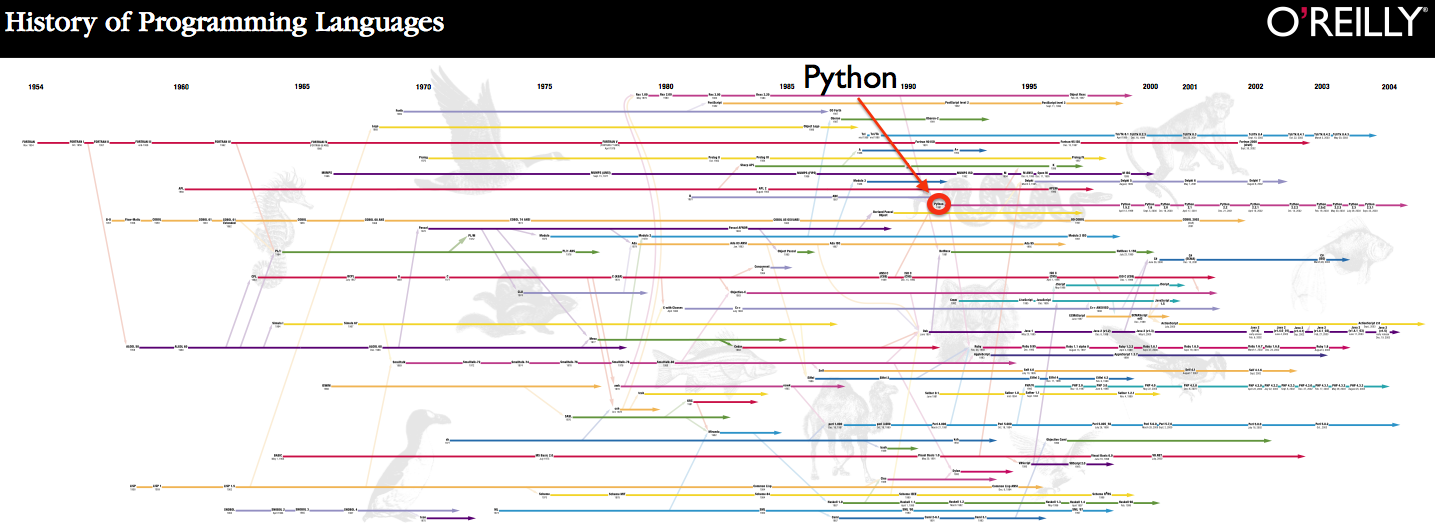
\includegraphics[width=300px]{ProgrammingLanguagesPoster-AnnotatedCropped.png} \\
    \tiny 
    Image credit: O'Reilly (\href{http://oreilly.com/news/graphics/prog\_lang\_poster.pdf}{http://oreilly.com/news/graphics/prog\_lang\_poster.pdf})
  \end{center}
\end{frame}

\begin{frame}
  \frametitle{Thanks!}
  \begin{itemize}
    \item We hope this little taste of the joys of programming whetted your appetite -- if so, this is the best place in the world to be.
    \item If you have any questions about Python, programming, or computer science in general, feel free to email either of us.
    \item Anshul: \href{mailto:nigham@gmail.com}{anshul@gmail.com}, Rob: \href{mailto:rpt@stanford.edu}{rpt@stanford.edu}.
    \item \texttt{\textbf{print 'Farewell, and godspeed!'}}
  \end{itemize}
\end{frame}



\end{document}
